\chapter{Análise sintática LR(1) e LALR}

\section{Introdução}\label{introduuxe7uxe3o}

No capítulo anterior, vimos os algoritmos LR(0) e SLR. O LR(0)
constrói um autômato cujos estados são conjuntos de itens da forma
\(A \to \beta . \gamma\) e preenche a tabela de ações sem considerar
o próximo token de entrada: toda entrada de reduce é preenchida para
\textbf{todos} os terminais.

Para motivar a necessidade de ir além do LR(0), considere a seguinte
gramática de expressões com recursão à \textbf{esquerda}:

\[
  \begin{array}{lcl}
    E & \to & E + T \mid T \\
    T & \to & n \mid ( E )
  \end{array}
\]

Essa gramática é LR(0): nenhum estado do autômato possui
simultaneamente um item completo e um item não completo com o mesmo
símbolo à direita do ponto. Por exemplo, o estado obtido após
reconhecer \(E\) no estado inicial contém:

\[
  \begin{array}{l}
    S' \to E . \\
    E \to E . + T
  \end{array}
\]

O primeiro item é aceitar em \(\$\) e o segundo é um shift em \(+\),
portanto não há conflito.

Agora modifiquemos a gramática para usar recursão à \textbf{direita}:

\[
  \begin{array}{lcl}
    E & \to & T + E \mid T \\
    T & \to & n \mid ( E )
  \end{array}
\]

Com essa mudança, o estado obtido após reconhecer \(T\) no estado
inicial passa a conter:

\[
  \begin{array}{l}
    E \to T . + E \\
    E \to T .
  \end{array}
\]

O item \(E \to T.\) está completo, então a construção LR(0) insere
uma ação de reduce \(E \to T\) para \textbf{todos} os terminais,
incluindo \(+\). Mas \(E \to T . + E\) exige uma ação de shift em
\(+\). Temos, portanto, um \textbf{conflito shift-reduce} em \(+\)
que o LR(0) não consegue resolver.

A raiz do problema é clara: quando o próximo token é \(+\), ainda é
possível completar \(E \to T + E\), portanto \textbf{não} devemos
reduzir. Quando o próximo token é \(\$\) ou \()\), não há como
continuar e \textbf{devemos} reduzir. Basta um único token de
lookahead para tomar a decisão correta.

Isso nos leva ao algoritmo \textbf{LR(1)}, que inclui em cada item
com um conjunto de lookaheads calculados localmente, não
globalmente como o SLR, tornando as ações de reduce precisas o
suficiente para resolver esses conflitos. O algoritmo
\textbf{LALR(1)} é uma variante prática do LR(1) que mantém o mesmo
número de estados do LR(0) ao fundir estados com o mesmo núcleo,
reunindo seus lookaheads.

\section{O Algoritmo LR(1)}

O algoritmo LR(1) constrói um autômato cujos estados representam o
progresso simultâneo de todas as derivações possíveis no contexto
atual. A cada estado está associado um conjunto de \textbf{itens
LR(1)}, cada um descrevendo o quanto de uma produção já foi analisado
e qual token pode legitimamente aparecer a seguir caso essa produção
seja completada. A partir desses estados, são extraídas as tabelas de
ações (shift, reduce, accept) e goto que guiam o analisador.

\subsection{Itens LR(1)}

Um \textbf{item LR(1)} tem a forma \([A \to \beta . \gamma, a]\). A
produção \(A \to \beta \gamma\) indica qual regra está sendo
reconhecida; o ponto separa a parte \(\beta\) já processada, que está
no topo da pilha, da parte \(\gamma\) que ainda está por vir na
entrada. O componente \(\alpha\) é o \textbf{lookahead}: um terminal (ou
\(\$\)) que pode aparecer imediatamente depois de toda a cadeia
derivada de \(A\) no contexto em que este item foi gerado. Ao
contrário do SLR, que calcula lookaheads globalmente usando conjuntos
FOLLOW, o LR(1) os deriva localmente a partir do contexto de cada item.

Quando o item está completo; isto é, quando \(\gamma =
\lambda\); o lookahead determina exatamente em qual coluna da
tabela de ações a redução \(A \to \beta\) deve ser inserida, evitando
conflitos com ações de shift que porventura também estejam presentes
no mesmo estado.

\subsection{Fechamento LR(1)}

O fechamento de um conjunto de itens LR(1) propaga as previsões de
forma análoga ao LR(0), mas agora carregando o lookahead correto para
cada nova previsão. Dado um item \([A \to \alpha . B \beta, a]\) em
que o próximo símbolo após o ponto é o não-terminal \(B\), para cada
produção \(B \to \gamma\) da gramática adicionamos ao conjunto o item
\([B \to . \gamma, b]\), onde \(b\) percorre todos os elementos de
\(\text{FIRST}(\beta\, a)\). Esse conjunto capta exatamente os
terminais que podem aparecer depois de \(B\) neste contexto: se
\(\beta\) não for anulável, são os primeiros de \(\beta\); se
\(\beta\) for anulável ou vazio, o próprio lookahead \(a\) também é
incluído. O processo é repetido até que nenhum item novo seja adicionado.

\subsection{Função goto LR(1)}

A transição entre estados é calculada pela função \(\text{goto}(I,
X)\), que recebe um estado \(I\) e um símbolo \(X\) (terminal ou
não-terminal) e devolve o estado alcançado após reconhecer \(X\).
Para construí-lo, tomamos todos os itens de \(I\) que têm \(X\)
imediatamente após o ponto, isto é, itens da forma \([A \to \alpha . X
\beta, a]\), avançamos o ponto para obter \([A \to \alpha X .
\beta, a]\) e calculamos o fechamento desse conjunto. O lookahead
\(a\) é transferido sem alteração, pois ele depende do contexto em
que o item foi criado, não do símbolo recém-reconhecido.

\subsection{Construção da Tabela LR(1)}

A construção começa com o estado inicial \(I_0\), obtido pelo
fechamento do item-semente \([S' \to . S, \$]\), onde \(S'\) é o
símbolo de partida aumentado. A partir de \(I_0\), novos estados são
gerados aplicando-se \(\text{goto}\) para cada símbolo que aparece à
direita de algum ponto no estado atual; esse processo é repetido para
todos os estados descobertos até que não haja mais novidades.

Com os estados em mãos, a tabela de ações é preenchida da seguinte
forma. Para cada item \([A \to \alpha . a \beta, b]\) em que \(a\) é
um terminal, insere-se um shift para o estado \(\text{goto}(I, a)\)
na entrada \(\text{action}[I, a]\). Para cada item completo \([A \to
\alpha ., a]\) com \(A \neq S'\), insere-se uma redução \(A \to
\alpha\) na entrada \(\text{action}[I, a]\): apenas na coluna do
lookahead \(a\), não em todas. Finalmente, quando o item \([S' \to S
., \$]\) está presente, registra-se accept em \(\text{action}[I,
\$]\). A tabela goto é preenchida com \(\text{goto}[I, B] =
\text{goto}(I, B)\) para cada não-terminal \(B\). Se nenhum par \((I,
a)\) receber duas ações distintas, a gramática é \textbf{LR(1)}.

\section{Exemplo: Tabela LR(1) para Expressões Aritméticas}

Considere a gramática de expressões com precedência:

\[
\begin{array}{lcl}
  E & \to & E + T \mid T \\
  T & \to & T \star F \mid F \\
  F & \to & ( E ) \mid n
\end{array}
\]

Aumentamos a gramática com \(S' \to E\).

\subsection{Construção dos estados}

\textbf{Estado 0}: fechamento de \(\{[S' \to . E, \$]\}\):

\[
\begin{array}{ll}
  S' \to . E    & \$ \\
  E \to . E + T & \$,+ \\
  E \to . T     & \$,+ \\
  T \to . T \star F & \$,+,\star \\
  T \to . F     & \$,+,\star \\
F \to . ( E ) & \$,+,\star,) \\
F \to . n     & \$,+,\star,)\\
\end{array}
\]

\textbf{Estado 1}: \(\text{goto}(I_0, E)\):

\[
\begin{array}{ll}
S' \to E . & \$ \\
E \to E . + T & \$,+
\end{array}
\]

\textbf{Estado 2}: \(\text{goto}(I_0, T)\):

\[
\begin{array}{ll}
E \to T . & \$,+ \\
T \to T . \star F & \$,+,\star
\end{array}
\]

\textbf{Estado 3}: \(\text{goto}(I_0, F)\):

\[
\begin{array}{ll}
T \to F . & \$,+,\star
\end{array}
\]

\textbf{Estado 4}: \(\text{goto}(I_0, ()\):

\[
\begin{array}{ll}
F \to ( . E ) & \$,+,\star,) \\
E \to . E + T & ),+ \\
E \to . T & ),+ \\
T \to . T * F & ),+,\star \\
T \to . F & ),+,\star \\
F \to . ( E ) & ),+,\star,( \\
F \to . n & ),+,\star,(
\end{array}
\]

\textbf{Estado 5}: \(\text{goto}(I_0, n)\):

\[
\begin{array}{ll}
F \to n . & \$,+,\star,)
\end{array}
\]

\textbf{Estado 6}: \(\text{goto}(I_1, +)\):

\[
\begin{array}{ll}
E \to E + . T & \$,+ \\
T \to . T * F & \$,+,\star \\
T \to . F & \$,+,\star \\
F \to . ( E ) & \$,+,\star,) \\
F \to . n & \$,+,\star,)
\end{array}
\]

\textbf{Estado 7}: \(\text{goto}(I_2, \star)\):

\[
\begin{array}{ll}
T \to T \star . F & \$,+,\star \\
F \to . ( E ) & \$,+,\star,) \\
F \to . n & \$,+,\star,)
\end{array}
\]

\textbf{Estado 8}: \(\text{goto}(I_4, E)\):

\[
\begin{array}{ll}
F \to ( E . ) & \$,+,\star,) \\
E \to E . + T & ),+
\end{array}
\]

\textbf{Estado 9}: \(\text{goto}(I_4, T)\):

\[
\begin{array}{ll}
E \to T . & ),+ \\
T \to T . \star F & ),+,\star
\end{array}
\]

\textbf{Estado 10}: \(\text{goto}(I_4, F)\) = \(\text{goto}(I_6,
F)\) = \(\text{goto}(I_7, F)\):

\[
\begin{array}{ll}
T \to F . & \$,+,\star,)
\end{array}
\]

(Estados 10--12 para os retornos dos subestados de 4 e 6 são
análogos; por simplicidade, listamos apenas os mais relevantes.)

\textbf{Estado 11}: \(\text{goto}(I_6, T)\):

\[
\begin{array}{ll}
E \to E + T . & \$,+ \\
T \to T . \star F & \$,+,\star
\end{array}
\]

\textbf{Estado 12}: \(\text{goto}(I_7, F)\):

\[
\begin{array}{ll}
T \to T \star F . & \$,+,\star,)
\end{array}
\]

\textbf{Estado 13}: \(\text{goto}(I_8, ))\):

\[
\begin{array}{ll}
F \to ( E ) . & \$,+,\star,)
\end{array}
\]

\textbf{Estado 14}: \(\text{goto}(I_8, +)\):

\[
\begin{array}{ll}
E \to E + . T & ),+ \\
T \to . T \star F & ),+,\star \\
T \to . F & ),+,\star \\
F \to . ( E ) & ),+,\star,( \\
F \to . n & ),+,\star,(
\end{array}
\]

\textbf{Estado 15}: \(\text{goto}(I_9, \star)\):

\[
\begin{array}{ll}
T \to T \star . F & ),+,\star \\
F \to . ( E ) & ),+,\star,( \\
F \to . n & ),+,\star,(
\end{array}
\]

\subsection{Tabela LR(1)}\label{tabela-lr1}

Os estados com itens completos têm reduções restritas aos lookaheads do item:

\begin{table}[H]
\begin{tabular}{@{}llllllllll@{}}
\toprule
Estado & n & + & $\star$ & ( & ) & \$ & E & T & F \\
\midrule
0 & s5 & & & s4 & & & 1 & 2 & 3 \\
1 & & s6 & & & & acc & & & \\
2 & & r E→T & s7 & & & r E→T & & & \\
3 & & r T→F & r T→F & & & r T→F & & & \\
4 & s5 & & & s4 & & & 8 & 9 & 3 \\
5 & & r F→n & r F→n & & r F→n & r F→n & & & \\
6 & s5 & & & s4 & & & & 11 & 10 \\
7 & s5 & & & s4 & & & & & 12 \\
8 & & s14 & & & s13 & & & & \\
9 & & r E→T & s15 & & r E→T & & & & \\
10 & & r T→F & r T→F & & r T→F & r T→F & & & \\
11 & & r E→E+T & s7 & & & r E→E+T & & & \\
12 & & r T→T*F & r T→T*F & & & r T→T*F & & & \\
13 & & r F→(E) & r F→(E) & & r F→(E) & r F→(E) & & & \\
14 & s5 & & & s4 & & & & 16 & 10 \\
15 & s5 & & & s4 & & & & & 17 \\
\bottomrule
\end{tabular}
\centering
\end{table}

(Estados 16 e 17 são análogos a 11 e 12, mas com lookaheads \(\{),+\}\).)

Observe que cada ação de reduce aparece apenas nas colunas
correspondentes ao lookahead do item, não em todas as colunas como no
LR(0). Isso evita conflitos que o SLR não conseguiria resolver quando
o conjunto FOLLOW é impreciso.

\section{O Algoritmo LALR(1)}

O LALR(1) (Look-Ahead LR) é uma simplificação prática do LR(1) que
reduz o número de estados sem abrir mão dos lookaheads locais. A
ideia central é observar que vários estados LR(1) distintos
compartilham o mesmo \textbf{núcleo}; isto é, os mesmos itens
quando ignoramos os lookaheads; e podem ser fundidos em um único
estado sem comprometer a correção do analisador na maioria das
gramáticas de interesse prático.

\subsection{Motivação}

O LR(1) resolve conflitos ao custo de multiplicar estados: dois
contextos diferentes que levam ao mesmo conjunto de itens LR(0) geram
estados LR(1) distintos porque seus lookaheads diferem. Na gramática
de expressões acima, por exemplo, os estados 3 e 10 têm o mesmo
núcleo \(T \to F .\), mas lookaheads diferentes: o estado 3,
originado fora de parênteses, carrega \(\{\$, +, \star\}\), enquanto
o estado 10, originado dentro de parênteses, carrega \(\{\$, +,
\star, )\}\). Para gramáticas de linguagens de programação realistas,
essa duplicação pode fazer o número de estados LR(1) ser uma ordem de
grandeza maior do que o número de estados LR(0), tornando as tabelas
proibitivamente grandes.

\subsection{Fusão de Estados}

O LALR(1) contorna esse problema fundindo todos os estados LR(1) que
compartilham o mesmo núcleo. O estado resultante reúne os lookaheads
de todos os estados fundidos, tomando a união dos conjuntos. Todas as
transições que apontavam para qualquer um dos estados originais
passam a apontar para o estado fundido. Como o núcleo (e portanto
a estrutura de shift e goto) é idêntico em todos os estados
mesclados, as transições permanecem consistentes após a fusão.

O único risco introduzido pela fusão é o surgimento de conflitos
reduce-reduce: se dois itens completos com o mesmo núcleo tinham
lookaheads disjuntos antes da fusão, sua união pode fazer com que
ambos reivindiquem a mesma entrada na tabela de ações. Quando isso
ocorre, a gramática é LR(1) mas não LALR(1). Vale notar que conflitos
shift-reduce nunca são introduzidos pela fusão: um shift é
determinado pelo núcleo do item, não pelo lookahead, de modo que um
conflito desse tipo no estado fundido já existiria nos estados LR(1) originais.

\subsection{Construção da Tabela LALR(1)}

Na prática, a tabela LALR(1) é obtida calculando-se primeiro todos os
estados LR(1), agrupando os que têm o mesmo núcleo e unindo seus
lookaheads. A tabela de ações e goto é então preenchida sobre os
estados fundidos exatamente da mesma forma que no LR(1): shifts são
determinados pelo núcleo do item, reduces são restritos ao lookahead
do item completo e accept ocorre ao atingir o item \([S' \to S .,
\$]\). O resultado é um analisador com o mesmo número de estados do
LR(0) e lookaheads mais precisos que o SLR.

\section{Exemplo: Tabela LALR(1) para Expressões Aritméticas}

Retomamos a mesma gramática de expressões do exemplo anterior.

\subsection{Identificação de estados com o mesmo núcleo}

Comparando os estados LR(1) construídos acima, identificamos os
seguintes grupos com o mesmo núcleo:

\begin{table}[H]
\begin{tabular}{@{}lll@{}}
\toprule
Núcleo & Estados LR(1) & Lookaheads unidos \\
\midrule
$T \to F .$ & 3 e 10 & $\{\$,+,\star,)\}$ \\
$E \to E + . T$, $T \to . T \star F$, $T \to . F$, \ldots & 6 e 14 &
$\{\$,+,)\}$ \\
$T \to T \star . F$, $F \to . (E)$, $F \to . n$ & 7 e 15 & $\{\$,+,\star,)\}$ \\
$E \to E + T .$, $T \to T . \star F$ & 11 e 16 & $\{\$,+,)\}$ \\
$T \to T \star F .$ & 12 e 17 & $\{\$,+,\star,)\}$ \\
\bottomrule
\end{tabular}
\centering
\end{table}

Os demais estados (0, 1, 2, 4, 5, 8, 9, 13) têm núcleos únicos e não
são fundidos.

Após a fusão, os estados LALR são nomeados como: \textbf{0, 1, 2,
3+10, 4, 5, 6+14, 7+15, 8, 9, 11+16, 12+17, 13}.

\subsection{Estados LALR resultantes}

\textbf{Estado 3+10} (fusão de 3 e 10):

\[
\begin{array}{ll}
T \to F . & \$,+,\star,)
\end{array}
\]

\textbf{Estado 6+14} (fusão de 6 e 14):

\[
\begin{array}{ll}
E \to E + . T & \$,+,) \\
T \to . T \star F & \$,+,\star,) \\
T \to . F & \$,+,\star,) \\
F \to . ( E ) & \$,+,\star,),( \\
F \to . n & \$,+,\star,),(
\end{array}
\]

\textbf{Estado 7+15} (fusão de 7 e 15):

\[
\begin{array}{ll}
T \to T \star . F & \$,+,\star,) \\
F \to . ( E ) & \$,+,\star,),( \\
F \to . n & \$,+,\star,),(
\end{array}
\]

\textbf{Estado 11+16} (fusão de 11 e 16):

\[
\begin{array}{ll}
E \to E + T . & \$,+,) \\
T \to T . \star F & \$,+,\star,)
\end{array}
\]

\textbf{Estado 12+17} (fusão de 12 e 17):

\[
\begin{array}{ll}
T \to T \star F . & \$,+,\star,)
\end{array}
\]

\subsection{Tabela LALR(1)}

A tabela LALR é construída sobre os estados fundidos. Usamos nomes
curtos para os estados fundidos: \textbf{A} = 3+10, \textbf{B} =
6+14, \textbf{C} = 7+15, \textbf{D} = 11+16, \textbf{E} = 12+17.

\begin{table}[H]
\begin{tabular}{@{}llllllllll@{}}
\toprule
Estado & n & + & $\star$ & ( & ) & \$ & E & T & F \\
\midrule
0 & s5 & & & s4 & & & 1 & 2 & A \\
1 & & sB & & & & acc & & & \\
2 & & r E→T & sC & & & r E→T & & & \\
A & & r T→F & r T→F & & r T→F & r T→F & & & \\
4 & s5 & & & s4 & & & 8 & 9 & A \\
5 & & r F→n & r F→n & & r F→n & r F→n & & & \\
B & s5 & & & s4 & & & & D & A \\
C & s5 & & & s4 & & & & & E \\
8 & & sB & & & s13 & & & & \\
9 & & r E→T & sC & & r E→T & & & & \\
D & & r E→E+T & sC & & r E→E+T & r E→E+T & & & \\
E & & r T→T*F & r T→T*F & & r T→T*F & r T→T*F & & & \\
13 & & r F→(E) & r F→(E) & & r F→(E) & r F→(E) & & & \\
\bottomrule
\end{tabular}
\centering
\end{table}

Comparando com a tabela LR(1), a tabela LALR tem menos estados (13 em
vez de 17), mas as ações de reduce são ligeiramente mais
conservadoras do que no SLR; por exemplo, no estado \textbf{A}
(\(T \to F.\)), a ação de reduce agora inclui \()\) como lookahead, o
que é correto porque este estado resulta da fusão de um contexto
externo (estado 3) e de um contexto dentro de parênteses (estado 10).
Como nenhum conflito foi introduzido pela fusão, portanto essa
gramática é \textbf{LALR(1)}.

\section{Implementação}

Nesta seção descrevemos os principais tipos e funções das
implementações Haskell dos algoritmos de construção de tabela LR(1) e
LALR(1), presentes nos módulos
\begin{flushleft}
\verb|Parsing.LR.LR1.BuildTable| e\\
\verb|Parsing.LR.LALR.BuildTable|.
\end{flushleft}
Ambos compartilham a mesma representação de estados e reutilizam o
algoritmo de parsing genérico do módulo
\verb|Parsing.LR.LRParser|.

\subsection{LR(1)}

\subsubsection{Itens e estados}

Um item LR(1) \([A \to \beta . \gamma, a]\) é representado pelo tipo:

\begin{minted}{haskell}
data LR1Item = LR1Item
  { lr1LHS :: String    -- não-terminal do lado esquerdo
  , lr1Before :: [Symbol]  -- símbolos antes do ponto
  , lr1After :: [Symbol]  -- símbolos depois do ponto
  , lr1Lookahead :: String    -- token de lookahead ou "$"
  }
\end{minted}

O campo \haskell{lr1Lookahead} é o componente
essencial que distingue os itens LR(1) dos itens LR(0): ele registra
o terminal que pode aparecer imediatamente após uma redução por \(A
\to \beta\) neste contexto específico. Um estado LR(1) é simplesmente
um conjunto de itens:

\begin{minted}{haskell}
type LR1State = Set LR1Item
\end{minted}

\subsubsection{Fechamento}

A função \haskell{closure} implementa o fechamento de
um conjunto de itens LR(1). Para cada item \([A \to \alpha . B \beta,
a]\), ela prediz todos os itens \([B \to . \gamma, b]\) onde \(b \in
\text{FIRST}(\beta\,a)\). O cálculo de \(\text{FIRST}(\beta\,a)\) é
feito pela função auxiliar \haskell{lookaheadsFor}:

\begin{minted}{haskell}
lookaheadsFor :: Grammar -> FirstSet -> [Symbol] -> String -> [String]
lookaheadsFor g fs beta a =
    filter (/= "\\") $ firstForSequence g fs (beta ++ [Terminal a])
\end{minted}

Ela concatena \(\beta\) com o lookahead \(a\) tratado como terminal e
chama \haskell{firstForSequence}, que já lida com
anulabilidade: se \(\beta\) for anulável, \(a\) é incluído no
resultado; caso contrário, apenas \(\text{FIRST}(\beta)\) aparece. O
fechamento em si aplica essa lógica repetidamente, usando o ponto
fixo da função \haskell{fixedPoint}:

\begin{minted}{haskell}
closure :: Grammar -> FirstSet -> LR1State -> LR1State
closure g fs = fixedPoint step
  where
    step current = Set.union current newItems
      where
        newItems = Set.fromList $ concatMap expand (Set.toList current)
        expand item = case lr1After item of
            (NonTerminal b : beta) ->
                [ LR1Item b [] prod la
                | prod <- prods b
                , la   <- lookaheadsFor g fs beta (lr1Lookahead item)
                ]
            _ -> []
\end{minted}

\subsubsection{Função goto e construção dos estados}

A função \haskell{goto g fs state X} avança o ponto
nos itens que têm \(X\) após ele e calcula o fechamento do resultado,
preservando o lookahead de cada item:

\begin{minted}{haskell}
goto :: Grammar -> FirstSet -> LR1State -> Symbol -> LR1State
goto g fs items sym = closure g fs $ Set.fromList shifted
  where
    shifted = mapMaybe shiftItem (Set.toList items)
    shiftItem item = case lr1After item of
        (s : rest) | s == sym ->
            Just $ LR1Item (lr1LHS item) (lr1Before item ++ [s])
                           rest (lr1Lookahead item)
        _ -> Nothing
\end{minted}

O conjunto canônico de estados LR(1) é construído por uma BFS que
parte do fechamento do item-semente \([S' \to . S, \$]\) e expande
cada estado pelos símbolos que aparecem após algum ponto:

\begin{minted}{haskell}
buildLR1States :: Grammar -> [LR1State]
buildLR1States g = buildFrom [initial] [initial]
  where
    seed    = LR1Item "S'" [] [NonTerminal startSym] "$"
    initial = closure g' fs (Set.singleton seed)

    buildFrom seen [] = seen
    buildFrom seen (current : queue) =
        let newStates = [goto g' fs current sym | sym <- nextSymbols current]
            unseen    = filter (`notElem` seen) newStates
        in buildFrom (seen ++ unseen) (queue ++ unseen)
\end{minted}

\subsubsection{Tabela de ações}

A construção da tabela em
\haskell{buildLR1ParsingTable} distingue-se do LR(0)
apenas na etapa de reduce: em vez de inserir a redução em todos os
terminais, ela usa exclusivamente o lookahead do item completo:

\begin{minted}{haskell}
reduceA =
    [ ((i, lr1Lookahead item), Reduce (lr1LHS item) (lr1Before item))
    | item <- Set.toList st
    , null (lr1After item)
    , lr1LHS item /= "S'"
    ]
\end{minted}

Esse detalhe é exatamente o que torna o LR(1) mais preciso que o
LR(0) e o SLR: a decisão de reduzir \(A \to \beta\) depende do token
seguinte calculado localmente para aquele item, não de um conjunto
FOLLOW global.

\subsection{LALR(1)}

\subsubsection{Núcleo de um estado}

A ideia central do LALR(1) é identificar estados LR(1) com o mesmo
\textbf{núcleo}, o conjunto de itens sem os lookaheads, e
fundi-los. O núcleo de um item é representado pelo tipo:

\begin{minted}{haskell}
type ItemCore = (String, [Symbol], [Symbol])

itemCore :: LR1Item -> ItemCore
itemCore item = (lr1LHS item, lr1Before item, lr1After item)

stateCore :: LR1State -> Set ItemCore
stateCore = Set.map itemCore
\end{minted}

Dois estados com \haskell{stateCore s1 == stateCore} possuem
exatamente os mesmos itens LR(0) subjacentes e são
candidatos à fusão.

\subsubsection{Fusão de estados}

A função \haskell{mergeGroup} recebe um grupo de
estados LR(1) com o mesmo núcleo e produz um único estado cujos itens
têm os lookaheads da \textbf{união} de todos os estados do grupo:

\begin{minted}{haskell}
mergeGroup :: [LR1State] -> LR1State
mergeGroup group =
    let byCore = Map.fromListWith Set.union
                   [(itemCore i, Set.singleton (lr1Lookahead i))
                   | i <- concatMap Set.toList group]
    in Set.fromList
         [LR1Item lhs before after la
         | ((lhs, before, after), las) <- Map.toList byCore
         , la <- Set.toList las]
\end{minted}

\subsubsection{Construção dos estados LALR}

A função \haskell{buildLALRStates} constrói o
conjunto canônico de estados LALR em três passos: primeiro chama
\haskell{buildLR1States} para obter todos os estados
LR(1); depois agrupa-os por núcleo, preservando a ordem de primeira
ocorrência de cada núcleo (o que faz os índices LALR coincidirem com
os índices LR(0)/SLR); por fim, funde cada grupo com
\haskell{mergeGroup}:

\begin{minted}{haskell}
buildLALRStates :: Grammar -> [LR1State]
buildLALRStates g =
    let lr1States = buildLR1States g
        coreOrder = nub (map stateCore lr1States)
        grouped   = Map.fromListWith (++)
                      [(stateCore s, [s]) | s <- lr1States]
    in [mergeGroup (grouped Map.! core) | core <- coreOrder]
\end{minted}

\subsubsection{Tabela e busca por núcleo}

A tabela LALR é construída exatamente como a tabela LR(1), mas as
transições são resolvidas por \textbf{correspondência de núcleo} em
vez de igualdade exata. Isso é necessário porque
\haskell{goto g' fs mergedState X} devolve um estado
LR(1) intermediário que pode não estar diretamente na lista de
estados LALR; o estado destino correto é aquele cujo núcleo coincide:

\begin{minted}{haskell}
findLALRStateIndex :: [LR1State] -> LR1State -> Maybe Int
findLALRStateIndex sts target =
    findIndex (\s -> stateCore s == stateCore target) sts
\end{minted}

Com isso, as entradas de shift e goto da tabela LALR apontam sempre
para estados fundidos, e as entradas de reduce usam os lookaheads
ampliados pela fusão: mais precisos que o FOLLOW global do SLR,
mas possivelmente mais amplos que os lookaheads originais do LR(1).

\section{Comparando algoritmos de análise sintática}

Os analisadores de Earley são os mais poderosos que já vimos: eles
podem reconhecer qualquer gramática, incluindo gramáticas ambíguas.
Eles podem até reconhecer línguagens ambíguas, línguagens para as
quais não existe uma gramática não ambígua, como \(\{a^nb^mc^p\,|\,n
= m \lor m = p\}\). Os analisadores de Earley exploram todo o poder
do autômato de pilha não determinístico (NPDA), que você pode
imaginar como um analisador shift-reduce com um oráculo indicando o
que fazer em caso de conflitos.

Parsing expression grammars permitem expressar gramáticas para
linguagens que não são livres de contexto, como \(\{a^nb^nc^n\,|\, n
\geq 0\}\). Porém, não se sabe se existem PEGs para linguagens livres
de contexto simples: como a linguagem de palíndromos. PEGs possuem a
vantagem de não possuir problemas de ambiguidade mas introduzem
dificuldades que não estão presentes em especificações baseadas
em gramáticas.

Algoritmos baseados em tabelas (LL(1), LR(1) e LALR) podem ser
caracterizados pelo seguinte diagrama, que demonstra a relação entre
diferentes classes de linguagens livres de contexto.

\begin{figure}[H]
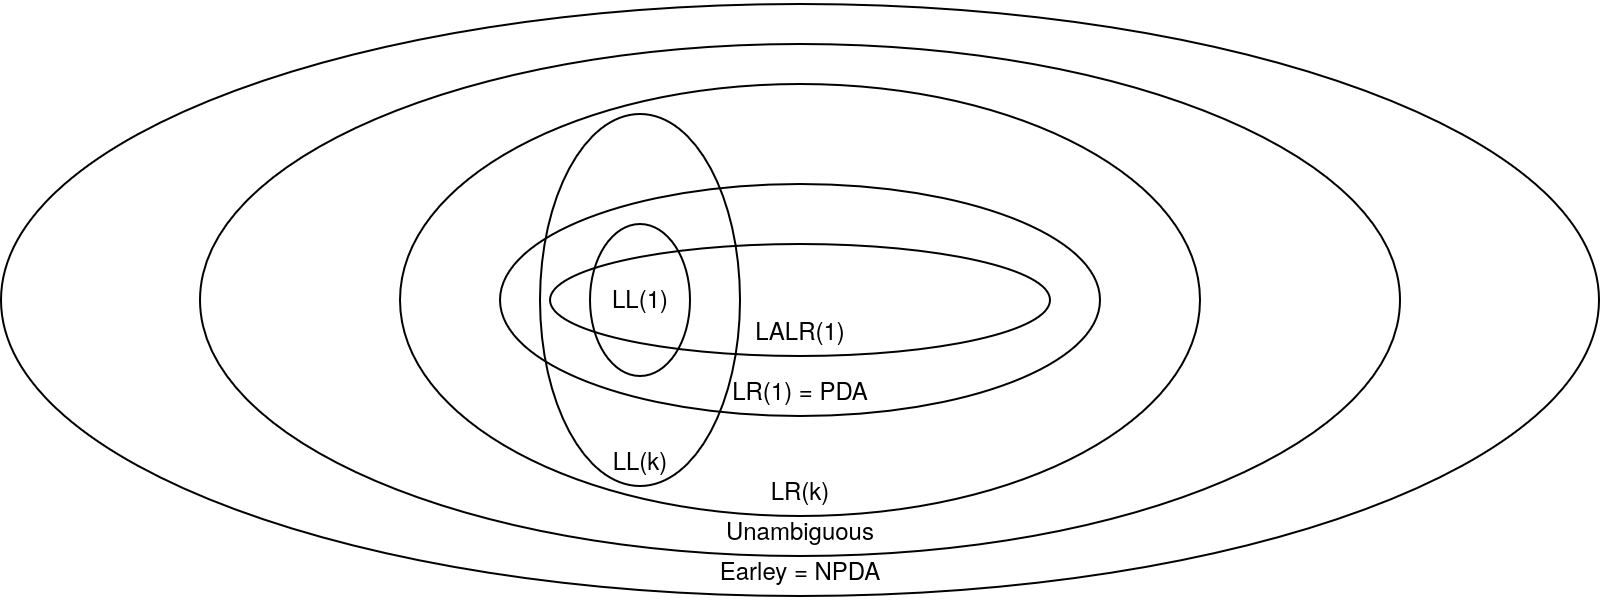
\includegraphics[scale=0.25]{chapters/grammars.png}
\centering
\end{figure}

\section{Conclusão}

Os algoritmos LR(1) e LALR(1) estendem o LR(0) e o SLR ao associar
lookaheads \textbf{locais} a cada item, em vez de usar o conjunto
FOLLOW global. O LR(1) é o mais preciso, mas gera o maior número de
estados. O LALR(1) oferece um equilíbrio excelente: funde estados
LR(1) com o mesmo núcleo, mantendo o número de estados igual ao
LR(0)/SLR e os lookaheads mais precisos que o SLR. Por isso, o
LALR(1) é o algoritmo de escolha para a maioria dos geradores de
analisadores sintáticos práticos.
